\documentclass{sig-alternate}

\usepackage{amsmath,amssymb}
\usepackage{stmaryrd}
\usepackage{graphicx}
\usepackage{color}

\newcommand{\longversion}[1]{}
\newcommand{\comment}[1]{}
\newcommand{\tinysection}[1]{\vspace{0.5mm}\noindent{\bf #1.}}
\newcommand{\tuple}[1]{{\langle#1\rangle}}
\newcommand{\todo}[1]{\textcolor{red}{#1}}
\newcommand{\note}[1]{\textcolor{blue}{#1}}


\begin{document}
\title{DBToaster: Agile Views in a\\Dynamic Data Management System}
\numberofauthors{3}
\author{
\alignauthor
Oliver Kennedy\thanks{Also Dept.\ of Computer Science, Cornell University.}\\
%    \affaddr{\'Ecole Polytechnique F\'ed\'erale de Lausanne} \\
    \affaddr{EPFL}
%    \affaddr{Lausanne, Switzerland}
    \email{oliver.kennedy@epfl.ch}
\alignauthor
Yanif Ahmad\\
    \affaddr{Johns Hopkins University}
%    \affaddr{Baltimore, MD}
    \email{yanif@cs.jhu.edu}
\alignauthor
Christoph Koch\\
    \affaddr{EPFL}
    % \affaddr{\'Ecole Polytechnique F\'ed\'erale de Lausanne} \\
    %\affaddr{Lausanne, Switzerland}
    \email{christoph.koch@epfl.ch}
}
\maketitle

\begin{abstract}
This paper calls for a new breed of lightweight systems --
{\em dynamic data management systems (DDMS)}\/.
In a nutshell,
a DDMS manages large {\em dynamic data structures}\/ with 
{\em agile, frequently fresh views}\/, and provides a facility for monitoring
these views and triggering application-level events.
%
We motivate DDMS with applications in large-scale data analytics
including data warehousing, and high-frequency algorithmic trading,
and compare them to more traditional data management systems 
architectures.
%such as DBMS and data stream processors.
%
We describe the DBToaster project, which is an ongoing effort to
develop a prototype DDMS system. We describe its architecture
design, techniques for high-frequency incremental view maintenance,
storage, scaling up by parallelization, and
the various key challenges to overcome to make DDMS a reality.
\end{abstract}


It is immediately plausible that one can do better than re-evaluate a query from scratch whenever the database changes a little. Incremental view maintenance (IVM) capitalizes on this insight \cite{DBLP:journals/tods/BunemanC79,DBLP:conf/sigmod/ShmueliI84,DBLP:conf/sigmod/BlakeleyLT86,roussopoulos-tods:91,DBLP:conf/vldb/CeriW91,DBLP:conf/deductive/GuptaKM92,DBLP:conf/sigmod/GuptaMS93,griffin-sigmod:95,yan-vldb:95,colby-sigmod:96,GHJ1996,kotidis-tods:01}. It is a solid, settled technique that has been implemented in many commercial DBMS, but has seen little new research activity in recent years and has gathered a little dust.

Now there is an exciting and potentially game-changing new development \cite{ahmad-vldb:09, koch-pods:10, kennedy-ahmad-koch-cidr:11}, an extreme form of IVM where all query evaluation work reduces to adding data (updates or materialized query results) to other materialized query results.  No join processing or anything semantically equivalent happens at any stage of processing. This works for a fragment of SQL with equijoins and aggregation, but without inequality joins or nesting aggregates.


Let us digest this, because the last claim goes counter to query processing intuitions to the point of absurdity. The main idea is the following: Classical IVM revolves around the idea that a materialized view can be maintained under updates by evaluating a so-called delta query and adding its result to the materialized view. The delta query captures how the query result changes in response to a change in the database. The new observation is that the delta query can be materialized and incrementally maintained using the same idea, making use of a delta query to the delta query, which again can be materialized and incrementally maintained, and so on, recursively. This works for classes of queries whose deltas are in some way structurally simpler than the base queries (e.g. having fewer joins), allowing this recursive query transformation to terminate. (It does so with a final trivial $k$-th delta query that does not refer to the database at all.) Termination is ensured for select-project-join queries with certain forms of aggregation, but some other features of SQL (specifically aggregations nested in where-conditions) have to be excluded. 

So where do the joins go? They {\em really} go away, as a benefit of incremental computation. If we want to compute $(x+1)*y$ and know $x*y$ and $y$, we only need to add $y$ to $x*y$, and the multiplication goes away. This is what happens when incrementally maintaining a join, where the join takes the place of multiplication. The pattern just sketched in basic algebra is not just an intuition but exactly what happens, and \cite{koch-pods:10} develops the algebraic framework to formalize this. We observe that the symbol 1 above represents the update workload.  In the incremental query processing framework, it must be a {\em constant} number of tuples that are changed in each incrementation step.

\comment{
To the reader who still cannot accept that joins can be replaced by no joins, we observe that the history of all incremental updates to the materialized view taken together is still essentially an execution of a nested loops join, that is, overall the value $x*y$ is constructed by adding $x$ copies of $y$. So if we put all the work associated with the individual updates happening over time together, the join work is still done. But refreshing the view in response to a single update does not require joins.
}

On paper, this approach clearly dominates classical IVM: if classical IVM is a good idea, then doing it recursively is an even better idea: The same efficiency-improvement argument for incremental maintenance of the base query also applies to the delta query. Argued from the viewpoint that joins are expensive and this approach eliminates them, one should expect a potential for excellent query performance.

But does this expectation translate into real performance gains? A priori, the cost of the bulk addition of materialized views or the costs associated with storing and managing additional auxiliary materialized views (for delta queries) might be more considerable than expected.


\medskip


This paper presents the lessons learned in an effort to realize recursive IVM, spanning nearly three years of intense work, to generalize it to be applicable on all or most of SQL, and to understand its strengths and drawbacks.
The contributions of this paper are as follows.
\begin{itemize}
\item
Multilevel IVM bears the promise of providing materialized views of complex SQL queries, without
window semantics or other restrictions, at very high refresh rates. We start by showing that there is
a need for such functionality, creating a benchmark consisting of automated trading and ETL workloads.
We show that state of the art systems cannot deliver materialized views refreshed at the rates
that some application domains (algorithmic trading, real-time analytics) require.
This is the challenge we set ourselves for the techniques and system described in this paper.

\item
We develop the vision of multilevel IVM further into a workable system.
While the techniques of \cite{ahmad-vldb:09, koch-pods:10} as well as existing implementations of
IVM in commercial DBMS are very restricted and exclude nested queries and other features of SQL,
we create the machinery to perform IVM and even recursive IVM on most of SQL (with the exception of
support for null values). To do this, we generalize the techniques of \cite{ahmad-vldb:09, koch-pods:10}
to not always materialize full delta queries but instead subexpressions that allow us to perform
IVM and maximize the performance obtained. This leads us to a query optimizer in which
the materialization of subqueries is a degree of freedom in optimization, and can be applied anywhere
in the input query or the delta queries obtained by applying this optimization.

To put ourselves in the position of using such an optimizer, we have to create suitable
intermediate representations of queries that support binding patterns for sideways information
passing, we study when and how to efficiently initialize views, and present query decomposition
and factorization techniques that lead to efficient formulations of update triggers that refresh our
views.

\item
Once high-level trigger programs for refreshing views based on multilevel IVM have been created,
we compile them further into highly efficient machine code.
We present our techniques for achieving this, which make use of sophisticated deforestation and
fusion techniques from the compilers literature.

\item
We have implemented our compiler and performed extensive experimentation with it. Our experiments
indicate that frequently, particularly for queries that consist of many joins of nested aggregation
subqueries that are not correlated through subqueries, our compilation approach dominates the
state of the art, often by multiple orders of magnitude. There are also queries in our benchmark
on which our techniques do not fare well; these usually involve the creation and maintenance of huge
auxiliary views whose data is rarely used by other views. These scenarios could be much improved upon
by suitable garbage collection strategies on auxiliary views. This is future work, and we consider
it likely that once such a technique has been integrated into our compiler, it will outperform the
state-of-the-art on an even wider range of queries.
\end{itemize}


The structure of the paper follows the order of contribution just laid out.















\comment{
This paper presents the lessons learned in an effort to realize aggressive IVM as motivated above. It represents an effort spanning nearly three years of intense work, which demonstrates that there are considerable technical challenges to be resolved. These key challenges are described next.


{\bf Compilation of update trigger code.}
%
The work that has to take place to update one materialized view with another (i.e., an auxiliary view representing a delta) is conceptually very simple; it essentially consists of bulk-adding tuple multiplicities of one view to another.

This updating work to be performed is particularly well-behaved and can be exploited for efficient evaluation:
\comment{
As observed in \cite{koch-pods:10}, this work is highly data-parallel. While parallel query evaluation is not the focus of the present paper, the updating work to be performed is particularly well-behaved. This can be exploited for efficient evaluation:
}
Classical query engines employ interpretation and large-gra\-nu\-la\-ri\-ty query operators such as joins to execute query plans.
In the past, IVM has used such query engines to evaluate its delta queries.
Instead, it is natural to avoid both query operators and plan interpretation, and the conceptual simplicity of the required work calls for aggressive code inlining and the elimination of the usual overheads due to interpreted query evaluation. It leads us to the compilation of view refreshing to lightweight machine code.

A considerable challenge is to determine suitable intermediate representations of query expressions to be used in the compiler. Such expressions in general have complex binding patterns which represent information flow. In general, this flow is not exclusively bottom-up.
Examples include complex conditions and nested subqueries correlated with their superqueries. Such expressions have input variables, and can only be evaluated if values for these input variables are given. In general, such expressions have to be materialized, which causes difficulties: how to determine a suitable domain for these input variables for which to materialize the results of the expressions, how to represent and store such materialized structures, and how to dynamically maintain the domains of input variables as updates add previously unseen values.


{\bf Compiler optimizations.}
%
Naively materializing delta queries, their delta queries, and so on causes the materialized views of the higher deltas to have high arity: in fact, the dimensionality can be as high as the arity of the product of all the relations joined together in the input query. The resulting size of the materialized views is of course unacceptable. As observed earlier \cite{ahmad-vldb:09, koch-pods:10} though, the materialized views can be losslessly decomposed into small views: taking a delta each time eliminates some join constraints, turning the views indeed into products.

This calls for factorization and decomposition techniques without which this approach would not be workable. In turn, however, recursive decomposition of delta queries of the various trigger programs (for insertions into and deletions from the relations occurring in the query) may produce large numbers of highly redundant factor views. This makes it essential to aggressively perform common subexpression elimination as well as deforestation and fusion techniques from the compiler literature.

In our implementation and experimentation efforts, this turned out to be much more important for satisfactory performance of the system than expected: without these techniques, recursive compilation for IVM with factorization as described in \cite{koch-pods:10} can result in hundreds of views to be maintained for a large join query, most of which are redundant and can be eliminated.
\comment{
Common subexpression elimination has been studied in the context of multi-query optimization, but here it takes a much more central role: without it, query performance will deteriorate by orders of magnitude almost every time: This is true even though we are referring to the compilation products of a single query, not a workload of multiple queries whose naturalness, if the queries share many subqueries, is often debatable. Thus, optimizations which are typically associated with compilers for general-purpose programming languages rather than query optimizers take a central role.
}
\comment{
We have also learned that some of the natural optimizations used in compilers for general-purpose programming languages rather than query optimizers take a central role. In particular, certain types of common subexpression elimination, loop fusion and analogous deforestation techniques for aggregations, are key to obtaining acceptable performance.
}
However, several of these optimizations such as deforestation have no form of expression in high-level query plan formalisms used in classical query optimization or recursive IVM. Thus, more than one internal intermediate representation (IR) of code is necessary.

\comment{
Our experiences led to two functional followed by one imperative IR. The functional IRs are a cleaned-up form of the algebraic expressions based on rings of queries and databases from \cite{koch-pods:10}, followed by a lower-level, Haskell-like and nearly general functional programming language in which we perform further forms of fusion and deforestation. The imperative IR is used in the compiler backend before imperative code generation. \comment{It is used for further optimizations that cannot be naturally expressed in a functional IR.} Overall, this leads us to a multi-stage reference compiler architecture for optimizing compilation of database queries to imperative code that we believe is general and relevant outside the context of incremental computation (cf. also Delite \cite{delite:11}).
}


\comment{
{\bf Side effects and initial value computation.}
%
Recursive IVM creates challenges we have not seen sufficient study of before, although they occur in simpler form in previous data management architectures that combine updating with querying, such as OLTP systems and stream processors: It is the tension between the convenience of viewing queries as pure functions of the data, and the {\em side-effects} that are updates.
In recursive IVM, an update triggers a variety of computations -- queries -- on various levels of a hierarchy of materialized views; one such computation creates data that is stored and used by another. These interleaved computations conceptually are meant to happen together, and side-effects must be carefully orchestrated to ensure a consistent database state after each update.

\comment{
In the context of recursive IVM, an update triggers a variety of computations -- queries -- on various levels of a hierarchy of materialized views; one such computation creates data that is stored and used by another. Compared to active databases, where certain events can trigger a cascade of computations, in the context of recursive IVM we face additional challenges in that interrelated computations do not profit from the benefits of isolation and conceptual serialization due to transaction semantics. The interleaved computations conceptually are meant to happen together.
}

As mentioned above, we in general need to materialize query expressions with binding patterns: queries that have input variables whose values cannot be determined from the query itself. The dynamic extension of the domains of these input variables and the resulting augmentation of the materialized views requires special initialization code distinct from the incrementation code (the compiled delta queries); this adds additional subtle challenges to the compilation framework. Most importantly, deciding how the domains of input variables of a materialized view has to be extended and optimizing the resulting code requires an intricate analysis of side effects across the hierarchy of materialized views.
} % end comment


{\bf Extraction/materialization as a first-class citizen of query optimizers.}
%
As stated above, the framework of recursive IVM requires delta queries to be structurally simpler than the queries they are deltas to. This is not the case for full SQL. This calls for abstracting from the strict notion of recursive IVM discussed in \cite{ahmad-vldb:09, koch-pods:10}. The key rewriting is to extract and materialize a subquery for IVM. This rewriting can be performed at multiple places in the query, as well as in delta queries that are used to incrementally maintain the materialization. In \cite{ahmad-vldb:09, koch-pods:10} the extracted subquery is always the full query or a factor in its product decomposition. But this is really an arbitrary restriction which can be lifted without causing fundamental problems.

This turns our compilation task into one of generating query evaluation code using an optimizer that has an {\em extract/materialize operator} that can be applied anywhere in the query, subject to optimization decisions (which we know from the literature on answering queries using views) but which also further compiles the delta queries auxiliary to materialization.


\medskip

The structure of the paper is as follows. Next, in Section~\ref{sec:sota}, we provide further motivation for the study of multilevel IVM by demonstrating by experimentation that low-latency continuous queries from ETL, monitoring and computational finance cannot be easily expressed by or managed by classical stream processors, or any other kind of existing engine. 
In Section~\ref{sec:compiler}, we present our compilation approach in detail, covering the various stages of a compiler from multilevel
incremental view maintenance to code generation.
Section~\ref{sec:experiments} returns to experimentation, picking up where we left off at the end of Section~\ref{sec:sota}, with all current data management systems failing to provide satisfactory performance for frequently fresh views for the workload proposed there.
We conclude with Section~\ref{sec:conclusion}.
} % end comment



\section{DDMS Architecture}
\begin{figure}
\begin{center}
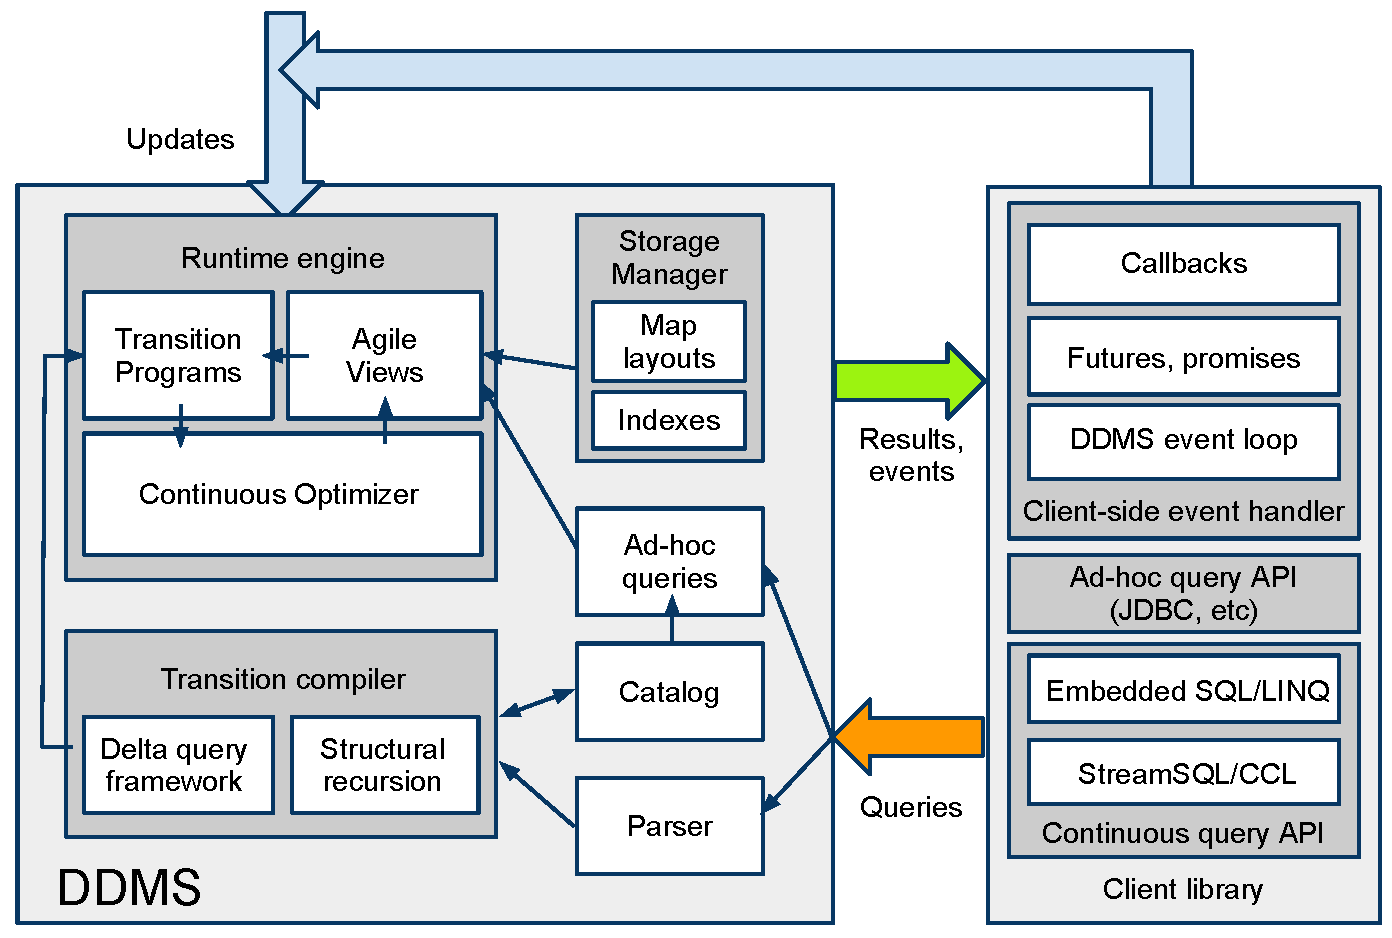
\includegraphics[width=3.3in]{graphics/CIDRarch.pdf}
\end{center}
\vspace*{-0.2in}
\caption{Dynamic Data Management System (DDMS) and Application Interface
Architecture}
\label{fig:ddmsarch}
\vspace*{-0.2in}
\end{figure}

We now examine the architecture of a DDMS, as illustrated in Figure
\ref{fig:ddmsarch}.  The core component of a DDMS is its runtime engine.  Unlike
a traditional database system where the same engine manages all database
instances, each individual DDMS execution runtime is constructed around a
specific set of queries provided by the client program (e.g., via SQL code
embedded inline in the program), each defining an \textit{agile view}.

\subsection{Application Interfaces}

The data that is processed by a DDMS arrives at the system in the form of an
update stream of tuple insertions, deletions and modifications. The stream need
not be ordered in any shape or form, and deletions are assumed to apply to
tuples that have already been seen at some arbitrary prior point on the stream.
Updates are fully processed on-the-fly, and their effects on agile views are
realised in atomic fashion, prior to working on any subsequent update. Depending
on the type of results requested by queries, any results arising from updates
will be directly forwarded to application code as agile views are maintained.

DBToaster provides a wide variety of client interfaces to issue queries and
obtain results from the DDMS, to reflect the diverse needs of applications built
on top of our tool. Today's stream processors tend to be black-box systems that
run completely decoupled from the application. Client libraries interact with
stream processors through remote procedure call abstractions, issuing queries
and new data through function calls, and either polling or being notified
whenever results appear on a queue that is associated with a TCP socket
connected to the stream processor.

In DBToaster, the set of agile views requested by clients, the \textit{visible
schema}, forms the primary read interface between client programs and the DDMS
runtime. Clients can submit queries for which the DDMS materializes an agile
view through three methods:
(1) a continuous query client API, as done with existing stream client
libraries, which sends a query string to the DDMS server for parsing,
compilation, and agile view construction. The query string may be specified in a
standard streaming language such as StreamSQL or CCL~\cite{jain-pvldb:08}. The
client may specify several ways to receive results, as seen below.
(2) an ad-hoc query client API, which issues a one-time query to the
DDMS, and returns the agile view as a datastructure to be used by the remainder
of the client program. This API may be used in both synchronous and
asynchronous modes, as indicated by the type of result requested. The query is
specified in standard SQL.
(3) an embedded language, whose syntax and data model are natural fits to the
host language in which the client application is written. Examples include
embedded SQL, and collection comprehension oriented approaches such as LINQ,
Links, and Ferry~\cite{meijer-sigmod:06,cooper-fmco:06,grust-sigmod:09}.
One interesting challenge with the embedded language approach is that of
enabling asynchronous event-driven programming. Whereas language embeddings
are natural for ad-hoc querying, we have yet to see these approaches
for stream processing.

Given these modes of issuing queries to the DDMS, our client interface supports
four methods of receiving results:
(1) callbacks, that can be specified as handlers as part of the continuous query
API. Callbacks receive a stream of query results, and are the simplest form of
result handlers that run to completion on query result events.  
(2) a DDMS event loop, which multiplexes result streams for multiple queries.
Applications may register callbacks to be executed on any result observed on the
event loop, allowing complex application behavior through dynamic
registration, observation and processing of results on the event loop.
(3) dynamic datastructures, which are read-only from the application
perspective. The datastructure appears as a native collection type in the host
language, facilitating natural access for the remainder of the program. Ad-hoc
queries use this method for results by default. Continuous queries may also use
this method in which case the datastructure acts as a proxy with accessors that
pull in any updates from the DDMS when invoked.
(4) promises and futures~\cite{Liskov:1988:PLS:53990.54016}, which provide a
push-based proxy datastructure for the
result. A future is an object whose value is not initially know and is provided
at a later time. A program using a query returning a future can use the future
as a native datatype, in essence constructing a client-side dataflow to be
executed whenever the future's value is bound. In our case, this occurs whenever
query results arrive from the DDMS. Language embedded stream processing can be
supported by futures, or program transformations to construct client side
dataflow, such as continuous passing style as found in the programming languages
literature~\cite{sussman-hsc:98}.


\comment{
An important distinction between the DDMS and a traditional DBMS is
that the DDMS treats both inputs (base relations in DBMS parlance) and agile views
(query outputs) as \textit{update streams} of tuple insertions, deletions and
revisions.  Updates are processed, and changes in the views are propagated
into the client.  If necessary, a DDMS runtime can also be instantiated with
support for ad-hoc queries.

The set of agile views requested by clients, the \textit{visible schema}, forms
the primary read interface between client programs and the DDMS runtime. This
interface comes in three flavors: (1) a push interface that invokes client
callbacks or schedules event handlers when a view in the visible schema changes,
(2) futures/promises representing queries over the visible schema that have not
yet been computed, or (3) read-only \textit{dynamic data structures}
representing each view in the visible schema.  One consequence of
limiting visibility into the database to the visible schema is that we are free
to represent a DDMS runtime's internal state in ways that are dramatically
different from a traditional DBMS.  We return to this observation later in the
paper.
}


\subsection{DDMS Internals}


%{\bf The runtime state machine}\/.
The internals of the runtime engine itself are best viewed through the lens of a
state machine.  Compared to similar abstractions for complex event
processors~\cite{agrawal-sigmod:08, demers-sigmod:07}, the state is
substantially larger. Conceptually, the state represents an entire
relational database and transitions represent changes in the base
relations: events in the update stream.



\tinysection{Compiling transitions}
Each transition causes maintenance work for our agile views, and just as
with incremental view maintenance, this work can be expressed as queries.
Maintenance can be aided by dynamic data structures, that is, additional agile
views making up the \textit{auxiliary schema}.
A DDMS is a long-running system, operating on a finite number of update streams.
This combination of characteristics naturally suggests \textit{compiling} and
specializing the runtime for each transition and associated maintenance
performed by a DDMS. The transition compiler generates lightweight transition
programs that can be invoked by the runtime engine with minimal overhead on the
arrival of events. We describe the compiler in further detail in Section
\ref{sec:dbtoaster}.




\tinysection{Storage management and ad-hoc query processing}
Given the instantiation of an auxiliary schema and agile views, a DDMS must
intelligently manage memory utilization, and memory-disk boundary as needed. The
storage manager of a DDMS is responsible for the efficient representation of
both the agile views, and any index structures required on these views.
Section~\ref{sec:storage} discusses the issue of indexing, as well as how views
are laid out onto disk. Supporting ad-hoc query processing turns out to be
relatively straightforward given the core of a DDMS continuously maintains agile
views. Ad-hoc queries can be rewritten to use agile views much in a similar
fashion to the materialized view usage problem in standard query optimization. A
key challenge here is how to ensure consistency, such that ad-hoc queries do not
use inconsistent agile views as update stream in and the DDMS performs
maintenance. On the other hand, we do not want ad-hoc queries to block the DDMS'
maintenance process and incur result delivery latency for continuous queries.
One option here is to maintain a list of undo actions for each ad-hoc query with
respect to agile view maintenance. This design is motivated by the fact that
continuous queries are the dominant mode of usage, and ad-hoc queries are
expected to occur less frequently, thus we bias the concurrency control burden
towards ad-hoc queries.





\comment{
Each transition is effectively a query for each view of interest. Though the
subqueries are simpler, it is not enough to make a DBMS-style query workload
tenable in a high-performance system.  However, instead of reevaluating the
subquery on every transition, we can the subquery as simply another agile view.
These views - the \textit{auxiliary schema} - are generated by a compilation
process discussed further in Section \ref{sec:dbtoaster}.
}

\comment{{\bf Space vs speed, partitioning and other optimizations}\/.}
\tinysection{Runtime adaptivity}
\comment{
The entire \textit{relevant} state of the database is completely expressed
through the auxiliary and visible schemas. However, substantial room exists for
optimization tradeoffs.
}
Significant improvements in just-in-time (JIT) compilation techniques means that
transition programs need not be rigid throughout the system's lifetime. A DDMS
includes a compiler and optimizer working in harmony, leveraging update stream
statistics to guide the decisions to be made across the database schema, state
and storage. For example, the compiler may choose to compute one or more views
on the fly, rather than maintaining it in order to keep expected space usage
within predefined bounds. The optimizer's decisions are made in terms of the
space being used, the cost of applying transitions on updates, as well as
information from a storage manager that aids in physical aspects of handling
large states, including implementing a variety of layouts and indexes to
facilitate processing.











\label{sec:overview}


\section{Realising Agile Views}
\label{sec:dbtoaster}
We present an example of designing a transition function between database
states, in this case focusing on dynamic data driving view maintenance of
standing queries comprising the visible schema. The underlying conceptual model
of a database management system as a state machine has driven our prior work on
this topic in the DBToaster project [REFS], and here we discuss how the concept
of transitioning entire database states has led to a novel view maintenance
algorithm. Furthermore the need to apply this transition with high frequency
motivates precomputing and compiling the transition function into extremely
efficient code.

This section is intended to convey that our database-as-state model can lead to
significant rethinking of existing methods throughout a data management system,
and novelty, algorithmically and architecturally, in designing a system to
handle dynamic data. Throughout this section, we use the term transition to
refer to both the update itself, and the work required to evolve the database
following the application of the update to base tables.

\vspace{1mm}
\subsection{View Maintenance in DBToaster}
Given a database state, existing view maintenance techniques will incrementally
handle transitions to another state for a given update. We can informally
represent this with a triple $\tuple{q,m,q'}$, corresponding to the view query,
the materialization of that query, and the delta query responsible for
maintaining the materialization.
\note{Should talk more about delta queries if you're going to make this the
first mention of it, i.e. with an example}
On an update, view maintenance performs the work: $m_{new} = m_{old} + q'(u)$,
and this is guaranteed to ensure $m_{new} = q(db_{new})$. That is, a
materialized view can be updated with the result of a delta query taking an
update $u$ as an argument, and the view maintenance technique must ensure the
updated view is equivalent to the query result on the modified database. Here,
the delta query can be thought of as a parameterized SQL query, with parameters
corresponding to attributes in the update.

With our conceptual model, we are able to make the
following key insight when taking a holistic approach with the state machine
model, namely that repeatedly applying the same transition with current
techniques results in significantly redundant work. While a transition results
in incremental processing in terms of the part of the database affected by the
update, it is not incremental with respect to the remainder of the database. The
transition evalutes delta queries from scratch on the remainder of the database,
rather than leveraging the fact that this remnant has not changed, and any work
done previously on that portion of the database can be reused.
\note{Diagram here:
\comment{states containing base relations and a query,
transitions for all base relations, each leading to another state. For one of these
neighboring states, we'll repeatedly apply the same transition, highlighting
that the remainder of the base tables do not change, yet the delta queries are
still evaluated from scratch.}
}

To facilitate reuse, we materialize the delta query over the remainder tables,
making it part of the auxiliary state of the database. We refer to this as the
view state, and it is used in our view maintenance approach. Subsequently our
transitions must maintain the view state, leading to the concept of higher-order
delta queries. Higher-order deltas are determined through a recursive processing
of materializing a delta query, and then incrementally maintaining the
materialized result (which would involve further materialization, and delta
queries and so on). That is we can define further triples,
$\tuple{q', m', q''}$, corresponding to the delta query, its materilization,
and a second-order delta query, and so on with $\tuple{q'',m'',q'''}$.
\note{Diagram here.}

This process does not continue forever and terminates given one important
property of computing delta queries: \textit{a delta query is often simpler than
its parent query}. In particular \textit{k}-th order delta query, $q^k$ has
fewer input relations than a \textit{k-1} order query $q^{k-1}$, but additional
parameters corresponding to attributes that are present in $q^{k-1}$. This
provides an informal overview of our view maintenance approach, and we present
an algorithm below to compute both the view state being materialized and the
higher-order delta queries that maintains the view state. The algorithm yields a
\textit{transition program}, essentially trigger function that efficiently
executes a transition from one database to another, including both the visible
and auxiliary state. For the view maintenance problem, the transition program is
simply a sequences of updates to materialized views by delta queries, each
update being of a different order.

\vspace{1mm}
\subsection{Compiling Queries to Transition Programs}
\noindent To present our algorithm, we first describe our query representation,
tailored for incremental processing, and a simple and powerful set of transformations
that we use to simplify and optimize queries.

\tinysection{Query Language}
\noindent Our query language is described by the following EBNF:

\def \calcsum{\mbox{Sum}}
\def\calceq{\mbox{{\tt =}}}
\def\calcgt{\mbox{{\tt >}}}
\def\calcgte{\mbox{{\tt >=}}}
\def\calclte{\mbox{{\tt <=}}}
\def\calclt{\mbox{{\tt <}}}

\def \q{q}
\def \qa{q_1}
\def \qb{q_2}
\def \v#1{\mbox{#1}}
\def \vv#1{\mbox{{\tiny #1}}}
\def \z{\mathbb{Z}}

\vspace{-3mm}
\begin{align*} 
\q \; \mbox{::-} &
  \;    c \;|\; x
  \;|\; R(\vec{x}) \;|\; m(\vec{x},\vec{y})
\\
| & \; \calcsum(\vec{x}, \q)
  \;|\; \q + \q \;|\; \q * \q  \;|\; -\q
  \;|\; \q \; \theta \; 0 \;|\; x := \q
\end{align*}

The grammar represents basic terms of queries such as constants, variables, and
relations $R$ (with attributes $\vec{x}$). We represent materialized views, $m$,
and refer to them as \textit{maps} since these are the underlying in-memory data
structures. Materialized views, or maps, are parameterized SQL queries that
accept parameters $\vec{x}$, and yield schema $\vec{y}$.
Specifically, a map is a \textit{materialized} parameterized query,
where we materialize for all parameter values seen during continuous query
execution (the \textit{active domain} of the parameter).
The intuition behind the representation of views as parameterized SQL comes from
our need to materialize delta queries, which have parameters according to the
update they handle.

For complex terms, the grammar captures sum aggregates
$Sum(\vec{x},q)$ with group-by attributes $\vec{x}$, three generalized
arithmetic operators, addition, multiplication and additive inverse, a
comparison operator ($\theta \in \{=,\neq,<,\leq,>,\geq\}$), and variable
assignment ($:=$). For readability, we write $\calcsum(\q)$ if an aggregate
has no group-bys, and simplify the syntax of comparison as $\theta(\q)$ since
the RHS is 0. 
Our language is quite rich, for example it can represent nested scalar
queries such as the VWAP query in Section [REF]:

\comment{
\begin{verbatim}
select sum(price * vol) from bids b0
where 0.25 * (select sum(b1.vol) from bids b1) >
     (select sum(b2.vol) from bids b2
      where b2.price > b0.price)
\end{verbatim}
}

\vspace{-3mm}
\begin{align*}
\calcsum(
& B(\v{P0,V0}) * \v{P0} * \v{V0} *\\
& \calcgt(0.25 * \calcsum(B(\v{P1,V1}) * \v{V1}) \\
& \qquad \; \; - \calcsum(B(\v{P2,V2}) * \v{V2} * \calcgt(\v{P2-P0}))))
\end{align*}

We briefly discuss expression semantics, starting with maps. Strictly speaking,
\textit{all of the expressions in our grammar (i.e. queries) represent maps},
and maps associate keys to values. Recall our analogy between maps
$m(\vec{x},\vec{y})$ and parameterized SQL queries. Map $m$ has a key
$\tuple{\vec{x},\vec{y}}$, namely the parameters (bound variables, which must be
provided when evaluating a parameterized query) and schema attributes (free
variables, returned by the query). For readability, we use a doubly-indexed map
notation, $m[\vec{x}][\vec{y}]$, instead of writing in pair notation throughout
$m[\tuple{\vec{x}, \vec{y}}]$. We define map values with a generalized multiset
relation [PODS REF] model of a database, where a relation $R$ is a map whose
value yields the cardinality of that tuple in a multiset.

We assume that the user queries provided as input to compilation contain no
maps, only relations and other terms as is standard in SQL. Our compilation
algorithm rewrites queries to include maps. Due to space constraints, we focus
on two arithmetic operations, addition and multiplication. First, we present an
example of addition:

\vspace{-7mm}
\begin{figure}[h]
\begin{minipage}{1in}
\[
\begin{array}{ll|ll|l}
\multicolumn{5}{c}{m1}\\
 a & c & b & d & \\
\hline
 1 & 1 & 2 & 1 & 3 \\
\comment{
 1 & 2 & 4 & 2 & 1 \\
 1 & 2 & 3 & 3 & 4 \\
}
 1 & 2 &   & 4 & 2
\end{array}
\]
\end{minipage}
+
\begin{minipage}{0.85in}
\[
\begin{array}{ll|l|l}
\multicolumn{4}{c}{m2}\\
 a & c & d & \\
\hline
 1 & 1 & 1 & 1 \\
 1 & 2 & 4 & 2 \\
\end{array}
\]
\end{minipage}
=
\begin{minipage}{1in}
\[
\begin{array}{ll|ll|l}
\multicolumn{5}{c}{m1 + m2}\\
 a & c & b & d & \\
\hline
 1 & 1 & 2 & 1 & 3 \\
 1 & 1 &   & 1 & 1 \\
\comment{
 1 & 2 & 4 & 2 & 1 \\
 1 & 2 & 3 & 3 & 4 \\
}
 1 & 2 &   & 4 & 4
\end{array}
\]
\end{minipage}
\end{figure}

\vspace{-3mm}
\noindent Above, we have two maps $m1, m2$, where blanks in columns represent
\textit{holes}. Holes are not the same as nulls, they determine when attributes
can be ignored for consistency across tuples.
\note{Explain consistency.}
Addition is a schemaless union where the result contains the union of
operand maps' parameters and result schemas, and adds the values of map entries.

Next, we discuss multiplication. Multiplication is the key
connective in our language since it performs binding propagation, similarly to
datalog, where one map's result schema contains attributes used for
another map's parameters, as seen in $m1[a][b1,b2] * m2[b2,c][d]$.
Here, $b2$ is propagated from map $m1$ to $m2$. The result of this
operation ensures consistency of $b2$ between maps $m1, m2$ (inconsistent
tuples are not included in the output), for example:

\vspace{-4mm}
\begin{figure}[h]
\begin{minipage}{1in}
\[
\begin{array}{l|ll|l}
\multicolumn{4}{c}{m1}\\
 a & b_1 & b_2 & \\
\hline
 1 & 2 & 4 & 3 \\
 2 & 4 & 1 & 1 \\
 2 & 3 & 2 & 4
\end{array}
\]
\end{minipage}
*
\begin{minipage}{0.85in}
\[
\begin{array}{ll|l|l}
\multicolumn{4}{c}{m2}\\
 b_2 & c & d & \\
\hline
 1 & 1 & 1 & 1 \\
 2 & 2 & 4 & 2 \\
\end{array}
\]
\end{minipage}
=
\begin{minipage}{1in}
\[
\begin{array}{ll|ll|l}
\multicolumn{5}{c}{m1 * m2}\\
 a & c & b_1 & d & \\
\hline
 2 & 1 & 4 & 1 & 1 \\
 2 & 2 & 3 & 4 & 8 \\
\end{array}
\]
\end{minipage}
\end{figure}

\vspace{-3mm}
\noindent Above, $b2$ is excluded from the result key since it is a propagated
attribute. The tuple $\tuple{a=1,b1=2,b2=4 \mapsto 3}$ in $m1$ does not
contribute to the result since there is no consistent value of $b2$ in $m2$.
Multiplication is a generalized equi-join, and in the absence of any
propagation, a generalized Cartesian product that operates on both levels of
maps.
\todo{Explain variables, i.e. we don't materialize attributes but these are
bound from the left.}
Binding propagation is critical for a few reasons: i) for
multiplication with variables, it allows a map's values to be combined with the
variable's value; ii) for multiplication with constraints, it yields maps
with 0-1 values indicating whether entries pass the constraint; iii) for
multiplication with other maps, where it facilitiates equi-joins and correlated
attributes in nested queries.


\comment{
We write these semantics as
$R := \tuple{} \mapsto \vec{x} \mapsto R(\vec{x})$, indicating the map has a key
with no parameters, schema $\vec{x}$, and value given by the cardinality $R(x)$
of the multiset $R$. The \textit{type} of the map is
$R : \tuple{} \mapsto \vec{x} \mapsto \z$, thus the semantics indicates the
result key, and the map value.

The semantics of constants and variables are: $c := \tuple{} \mapsto
\tuple{} \mapsto c$ and $Var(x) := \vec{b} \mapsto \tuple{} \mapsto \vec{b}(x)$.
The latter states that variables get their value from query parameters.
Due to space constraints, we briefly present the semantics of complex terms.


\vspace{-4mm}
\begin{align*}
\calcsum(\vec{y}, \q[\vec{x}][\vec{y}\vec{z}]) := & \;
\vec{x} \mapsto \vec{y} \mapsto \sum_{\vec{z}} \q
\\
\qa[\vec{u}][\vec{v}] + \qb[\vec{w}][\vec{x}] := & \;
\vec{y} \mapsto \vec{z} \mapsto
\qa[\vec{y}][\vec{z}] + \qb[\vec{y}][\vec{z}]
\\
& \mbox{ where $\vec{y} = \vec{u} \cup \vec{w}, \vec{z} = \vec{v} \cup \vec{x}$}
\\
-\q[\vec{x}][\vec{y}] := & \; \vec{x} \mapsto \vec{y} \mapsto -(\q)
\\
\q[\vec{x}][] \; \theta \; 0 := & \; \vec{x} \mapsto \tuple{} \mapsto
                    \begin{cases}
                    1 \ldots \q \; \theta \; 0\\
                    0 \ldots \mbox{otherwise.}
                    \end{cases}
\\
(x := \q[\vec{b}][]) := & \; \vec{b} \mapsto \tuple{x=q} \mapsto 1
\end{align*}

Above, we write typing constraints of subexpressions on the left-hand
side of semantics definitions. Thus a sum aggregate with group-by $\vec{y}$
over a map $q[\vec{x}][\vec{yz}]$ adds up values of $\vec{z}$. 
\note{Talk about consistency.}
The addition operator ($+$) is a schemaless union over both parameters and
result schema of its inputs. Additive inverse simply negates the map value,
preserving its type. Predicates yield maps with 0-1 values, and are constrained
to have no output schema. They are singletons, just like constants and
variables, and in this way, our language supports nested scalar queries such as
nested sum aggregates. Finally variable assignment $x := q$ yields a singleton
map with schema $x$, and key (of value) $q$. This leaves the multiplication
operator, which in our langauge is capable of propagating parameters, much like
datalog. Suppose we have: $\qa[\vec{u}][\vec{v}] * \qb[\vec{w}][\vec{x}] :=$

\vspace{-4mm}
\begin{align*}
& \vec{y} \mapsto
\sum_{\{y\} = \{u\} \Join \{w\}} 
\vec{z} \mapsto
  \sum_{\{z\} = \{v\} \Join \{x\}}
  \qa[\vec{y}][\vec{z}] * \qb[\vec{y}][\vec{z}]
\\
& \ldots \mbox{when $\vec{v} \cap \vec{w} = \emptyset$}
\\
& \vec{y} \mapsto
\sum_{\{y\} = \{u\} \Join \{b\}} 
\vec{z} \mapsto
  \sum_{\{z\} = \{v\} \Join \{ax\}}
  \qa[\vec{y}][\vec{z}] * \qb[\vec{y}][\vec{z}]
\\
& \ldots \mbox{otherwise, where $\vec{v} \cap \vec{w} = \vec{a}, 
\vec{w} - \vec{v} = \vec{b}$}
\end{align*}

Above, the first case describes when no propagation occurs. The result map has
parameters and schema according to the join of the operands' keys and value as a
product of operand values. In the second case we have propagation of the LHS
query's result schema being bound as parameters in the RHS query. Thus the
result map does not consider propagated attributes as parameters itself.
}


\vspace{0.5mm}
\tinysection{Query Transformations}
We present a set of query transformations, through examples for brevity, that
can be used by our algorithm to simplify and optimize queries.
\comment{
The first is a canonicalization of queries into a \textit{recursively
polynomial} form. A polynomial query is a query represented as a sum of
\textit{monomials}, where monomials are products of any other type of query
(constraints, aggregates, etc. but not sums or products). This is a polynomial
with two monomials:
\begin{align*}
\calcsum( & R(\v{A,B}) * S(\v{C,D}) * \calcgt(\v{B}-\v{C}) *
\calceq(\v{A}-\v{D})) * \\
& \calcsum(T(\v{E,F}) * \v{E}) + -\calcsum(U(\v{G,H}) * \calceq(\v{H}-5))
\end{align*}
The following query is not a polynomial:

$\calcsum(R(\v{A,B}) + (S(\v{C,D}) * \v{C})) *
 \calcsum(T(\v{E,F}) * \calceq(\v{E}-10))$

\noindent because of the addition inside the first sum aggregate. Due to nested
queries, we define our normal form recursively, where each nested
query is also in polynomial form. We require this normal form to easily apply
the following simplifications.
}

To simplify queries, we apply unification, which facilitates variable
elimination, and then factorization, which separates a complex monomial into a
product of simpler monomials. First we give an example of unification and
variable elimination: \todo{xxx}

Now, we demonstrate factorization: \todo{xxx}

Above, \todo{description}

Finally, we present a transformation related to binding propagation, called
preaggregation. This ensures that our product operation propagates the minimal
number of variables, when considering a left-associative multiplication.
The VWAP query [REF in this section] would result in the following after
preaggregation:

\vspace{-3mm}
\begin{align*}
\calcsum(
& \calcsum(\tuple{\v{P0}}, B(\v{P0,V0}) * \v{P0} * \v{V0}) *\\
& \calcgt(0.25 * \calcsum(B(\v{P1,V1}) * \v{V1}) \\
& \qquad \; \; - \calcsum(B(\v{P2,V2}) * \v{V2} * \calcgt(\v{P2-P0})))
\end{align*}

\noindent In contrast to the original VWAP query, the subexpression
$B(\v{P0,V0}) * \v{P0} * \v{V0}$ is preaggregated by an enclosing sum aggregate
to only propagate $\v{P0}$ to the nested query, and not $\v{P0,V0}$.

\tinysection{Incremental Processing}
So far, we have described queries, with no mention of incremental processing. We
now describe a transformation to compute the \textit{delta} of a query, which
computes the increment for a query given an update to one of its input
relations. The \textit{delta is itself a query}, and conceptually
is derived by replacing the input relation being updated with a set of
parameters. These parameters are passed to the transition program, thus the
delta query can be thought of as a parameterized SQL query. Our transformation
rules for computing delta queries are:

\vspace{-3mm}
\begin{align*}
\comment{
\Delta_{+R(\vec{x} \mapsto \vec{t})} c := & \; 0
\\
\Delta_{+R(\vec{x} \mapsto \vec{t})} Var(y) := & \; 0
\\
}
\Delta_{+R(\vec{x} \mapsto \vec{t})} R(\vec{x}) := & \;
\prod_i^{sch(\vec{x})} x_i := t_i
\\
\comment{
\Delta_{+R(\vec{x} \mapsto \vec{t})} S(\vec{y}) := & \; 0
\\
}
\Delta_{+R(\vec{x} \mapsto \vec{t})}
\calcsum(\vec{x},\q) := & \; \calcsum(\vec{x},\Delta\q)
\\
\Delta_{+R(\vec{x} \mapsto \vec{t})} (\qa + \qb) := & \;
(\Delta\qa + \Delta\qb)
\\
\Delta_{+R(\vec{x} \mapsto \vec{t})} (\qa * \qb) := & \;
(\Delta \qa * \qb) +
(\qa * \Delta \qb) +
(\Delta \qa * \Delta \qb)
\\
\Delta_{+R(\vec{x} \mapsto \vec{t})} \theta(\q) := & \;
(\theta(\q + \Delta \q) * \overline{\theta}(\q)) -
(\overline{\theta}(\q+\Delta \q) * \theta(\q))
\\
\Delta_{+R(\vec{x} \mapsto \vec{t})} -\q := & \;
    -(\Delta \q)
\\
\Delta_{+R(\vec{x} \mapsto \vec{t})} (x := \q) := & \;
    (x := \Delta \q)
\end{align*}

The above top-down rules specify deltas for complex terms. In addition, deltas
of constants and variables yield 0, and the delta of a relation other than the
one being updated also yields 0 (i.e. the rule: $\Delta_{+R(\vec{x} \mapsto
\vec{t})} S(\vec{y}) := \; 0$). Also note, we have no rule for maps, since maps
do not appear in user queries. All of these transformations are applied before
our algorithm introduces maps. These rules are similar to those from
incremental view maintenance, with the exception of our rule for constraints,
which can handle nested queries. To the best of our knowledge, we have not seen
this addressed before. We wrap up deltas with two insights: i) delta queries are
nearly always \textit{simpler} than their parent queries, with the exception of
nested queries; ii) queries are closed under taking deltas, that is our delta
queries are in the same language fragment, they too are SQL queries.
We will need to build a main-memory SQL engine, and we talk about novel
approaches with code generation in our algorithm.

\tinysection{Compiling Transition Programs}
We can now piece together the various transformations above, to perform
\textit{recursive query compilation}. Our algorithm produces transition
programs, which have the following grammar:

\vspace{-3mm}
\begin{align*}
M3    & \; \mbox{::= on (insert$|$delete$|$update) }
           R(\vec{x}\vec{y}) \; \{ stmt^* \}\\
\comment{event & \; \mbox{::= insert $|$ delete}\\}
stmt  & \; \mbox{::= } m[\vec{x}\vec{i}][\vec{y}\vec{j}] \;
                       \mbox{{\tt $\pm$=}} \; \q\\
\end{align*}

\noindent Transition programs as simple sequences of map updates.
Here $\q$ refers to our query representation, resulting from the fact that
queries are closed under deltas. Above, the function has arguments
$\vec{x}\vec{y}$, referring to the transition parameters which will be used in
both the LHS map of the statement as can be seen, as well as in the RHS delta
query.
The transition program for VWAP is:

\begin{verbatim}
on_insert_bids(p, v) {
  // aliases due to limited presentation space.
  // these are inlined in our code.
  c1 = 4*q2[p][] - q1[][];
  c2 = 4*q2[p][] - q1[][]+v;
  c3(d) = fun d -> 4*q2[d][] - q1[][];
  c4(d) = fun d -> 4*(q2[d][]+(v*<(d-p)))-q1[][]+v);

  // q1     = sum v from bids
  // q2(p2) = sum v from bids where p > p2
  // q3     = sum p*v from bids group by p
  // q4     = sum v from bids group by p
  q[][]   += p * v * >(c1);  
  q[][]   += sum(d, q3[][d] * <=(c3(d)) * >(c4(d));
  q[][]   -= sum(d, q3[][d] * >(c3(d)) * <=(c4(d));
  q[][]   += p * v * <=(c1) * >(c2);
  q[][]   -= p * v * >(c1) * <=(c2);
  q1[][]  += v; q2[d][] += v * >(p-d); 
  q3[][p] += p * v; q4[][p] += v;
}
\end{verbatim}

In our implementation, the RHS queries in these statements are compiled down to
C code (omitted for space).
\todo{Talk about higher-order deltas here.}
One issue that arises is on the arrival of new parameter values which we have
not seen previously, for both map lookups (map accesses in the RHS queries) and
map updates (map accesses on the LHS of statements). This requires
\textit{initial value computation}, which for queries with only simple equality
constraints has value 0, but in general requires evaluation of a parent query
instead of its delta. The above program omits initializers.

\def \alg         {{\bf algorithm}}
\def \algbegin    {{\bf begin}}
\def \algend      {{\bf end}}
\def \algforeach  {{\bf for each}}
\def \algdo       {{\bf do}}
\def \algdone     {{\bf done}}
\def \algreturn   {{\bf return}}
\def \algcomment#1{{\tt //} #1}

\def \codeforeach {{\tt for}}
\def \codev#1     {\mbox{{\tt #1}}}

A simplified algorithm for producing the above is:

\vspace{-1mm}
\begin{tabbing}
\alg\ Compile(\q: query, m: map name, $\vec{x}$: map keys) \\
\algcomment{returns triggers (a set of map update statements)}\\
\algcomment{for update events to relations in \q} \\
$\Gamma_{\q} := \Gamma$\\
\algforeach\ base relation $R$ in \q,
               $\pm$ in $\{\v{insert},\v{delete}\}$
\algdo \\
~~\= $\vec{t}$ := fresh variables for columns of $R$
     \algcomment{trigger args}\\
  \> $\vec{b} \; := \; \vec{t} \; \cup \; \vec{x}$
     $\qquad \qquad \qquad \qquad \qquad$ \algcomment{bound vars}\\
  \> $\v{\q}_{init}$ := MakeInitializer(\q)\\
  \> \algforeach\ $\v{q}_{m_i}$ in Monomialize($\Delta\v{q}$) \algdo\\
\>~~\= ($\partial\v{q}_i$, $\Gamma_i$) :=\=\ ExtractSimplerQuery($\vec{b}$,\\
  \>\>\> ~~ SimplifyQuery($\partial\v{q}_{m_i}$, $\vec{b}$))\\
  \>\> $\partial_{init} := $ MakeInitializer($\partial\v{\q} _i$)\\
  \>\> $\v{s}_i$ := \= EliminateLoops(MakeStmt(\\
  \>\>\> ~~\{\codeforeach\ $\vec{x} \in \codev{m} [\vec{x}]:$
  $\codev{m} [\vec{x}]\tuple{\v{\q}_{init}} \pm = $
  $\partial\codev{q} _{i}\tuple{\partial_{init}}$\}))\\
  \>\> triggers[$R$] := triggers[$R$] $\cup$ \todo{Annotate($\v{s}_i$)}\\
  \>\> $\Gamma := \Gamma \bigcup_i \Gamma_i$
  \ \ \ \ \algcomment{eliminates duplicate maps}\\
  \>\algdone\\
\algdone\\
\algforeach\ $(q, m[\vec{x}]) \in \Gamma - \Gamma_{\q}$ \algdo\\
  \> triggers := triggers $\bigcup_{R}$ Compile($q, m, \vec{x}$); \\
\comment{\algdone\\}
\algreturn\ triggers
\end{tabbing}

\todo{
\begin{itemize}
  \item Simplify compilation algorithm
  \item Describe additional steps beyond sequentially applying transformations
    \begin{itemize}
    \item loop var simplification
    \item initializer expression computation
    \end{itemize}
\end{itemize}
}

\tinysection{Towards a Framework for Optimizing Physical Engine Properties}
Our implementation of delta queries appearing on the RHS of statements uses an
restricted functional programming language, where we can apply
techniques from structural recursion [REF], prior to generating low-level code. 
Structural recursion enables optimizations of arbitrarily nested structures such
as sets, bags and lists, and while it might not immediately be clear how this
pertains to delta queries on maps, we provide the following insight:
\textit{structural recursion enables programmatic representation and
manipulation of numerous physical-level properties, such as tuple
construction and pipelining}.

Our delta queries consist of many maps used as inputs to cross products and
joins based on the presence of binding propagation in multiplications. In a
traditional DBMS engine treats, cross products and join operators work on
relations, to produce relations, ``flattening'' intermediate results into rows.
Column-stores have argued for the late materialization of tuples [REF: Abadi
ICDE 2007]. We produce intermediate results in a general nested form (think of
nested relations) which may include multiple levels of nesting after combining
several maps. Then, we can exploit structural recursion which critically makes
use of function composition and inlining, to programmatically control where, and
how much tuple construction we perform.

We show a structural recursion example for another physical-level transformation
on the following query: \todo{3-way join as binary join-tree w/ maps.}

We can transform this to: \todo{3 way join as 3 level nested loops w/ no
intermediates.} \todo{Describe benefits.}

To summarize, to the best of our knowledge, DBToaster incorporates the first
query representation (in functional form) for programmatic manipulation of
physical aspects of plans and operators. We can do this because we are reasoning
about query evaluation from a data structure perspective, not an operator
abstraction (which encapsulates and hides data structures).

\begin{itemize}
  \item Give two simplified examples of programs, one showing join tree,
  one showing multiway join.
  \item Mention tradeoffs in two programs.
\end{itemize}


\section{Managing Storage in DBToaster}
\label{sec:storage}
Typical DDMS workloads require large state, necessitating the use of more
intelligent storage techniques. Compared to traditional DBMS, DDMS have more
information to use when constructing a task-specific storage solution.

We now examine two components of DBToaster's solution to storage in a DDMS: (1)
The DBToaster compiler produces datastructures designed specifically for the
compiled DDMS' target query workload. (2) By analyzing the patterns with which
data is accessed, DBToaster constructs a data layout strategy (for pages on a
disk, servers in a cluster, etc...) that limits IO overhead.

\subsection{Datastructures}
DBToaster uses multi-key maps to represent materialized views, as seen in
Section~\ref{sec:compilation}. Furthermore, we discussed the need for iterating
over, that is performing \textit{partial lookups} of map entries while applying
updates. Recall line 2 in the code listing in Section~\ref{sec:compilation}.
This is a partial lookup on map $m_c$ with only {\tt ck} present from function
arguments. In addition to exact and partial lookups, we require maps to provide
range lookups due to inequality predicates in queries, while ensuring map
values correspond to aggregates.

\comment{
Regardless of whether data is stored in memory, on disk, or across an entire
cluster, efficient disk access begins with good representation.  As its data
storage primitive, DBToaster uses multi-key maps, which have thus far not been
formally defined.

Fundamentally, a multi-key map is a simple key-value store with structured
(i.e., schema-defined) keys and values, as well as some iteration capabilities. 
However, generated statements do not typically iterate over the entire
datastructure.  In the common case, statements iterate over keys matching a
selection predicate.  For example, when updating Section \ref{sec:dbtoaster}'s
$m_c$ after an insertion into \texttt{lineitem}, we iterate over all values
matching the predicate \texttt{@ok = orderkey}.

Though similar to relational tables in this respect, there are two subtle, but
critical differences: (1) The map's value at each point is defined not by the
data stored in it, but rather as a function (subquery) over the state of the
database.  (2) Unlike a relational table, where absent keys imply NULL values,
multi-key maps are defined for all keys conforming to the map's schema.

These two differences are closely related.  A map's value must be defined for
all keys, because all updates are specified as deltas.  In the absence of prior
state, this value can be derived from lower level maps, or the base relations. 
Interestingly, for non-nested queries without inequalities, this value always
begins at zero.  So long as the maps are maintained incrementally, we never need
to compute the initial value.

This functional view of maps paves the way for a range of entirely different
data representations: 
}

In their simplest form, out-of-core maps can be implemented by a simple
relational-style key-value store with secondary indices\cite{berkeleydb}.
\comment{
However, the map could simply act as an incrementally maintained cache.
Recently computed values are not only available for re-use, they are dynamically
updated as the underlying function gets new inputs.
}
Inequality predicates, and aggregations including such predicates, can be
implemented efficiently using maps that store cumulative
sums\cite{rangequeries}.  Maps can apply compression techniques to address
frequently repeating data.
\comment{
As another example, a probabilistic database built on top of a DDMS might use
maps representing regressions, a markov random field, a bayes nets, etc\ldots
}
DBToaster can customize the data structures backing each materialized view based
on statement-level information on accesses, applying static compile-time
techniques to construct specialized data structures.

With substantial specialization of data structures as part of compiling
transitions, DBToaster is free to consider a range of runtime issues in data
structure tuning and adaptation, including how to best perform fine-grained
operations such as incremental and partial
indexing~\cite{stonebreaker-sigrec:89}. The key challenge to be addressed is how
to provide data structures with a low practical update cost (avoiding expensive
index rebalancing and hash-table rebucketing) while gradually ensuring the
lookup requirements of our datastructures are ensured over time, amortizing data
structure construction with continuous query execution.


\subsection{Messaging, Storage and Partitioning}
Even with good datastructures, haphazard data placement leads to poor
performance.  Though precise workload data may not be available at compile time,
DBToaster optimizes the way it lays out its database across memory, a disk, or
even a server cluster, based on the query workload it is constructed with.  An
elegant abstraction for doing this is the \textit{messaging graph}.

Each transition function can be represented as a bipartite directed hypergraph;
nodes on the left represent portions of the database being read from, nodes on
the right represent a portions being written to, and each hyperedge represents
an independent subtask of the transition function.  An example is shown in
Figure \ref{fig:diag:messagingGraph}a.

\begin{figure}
\begin{center}
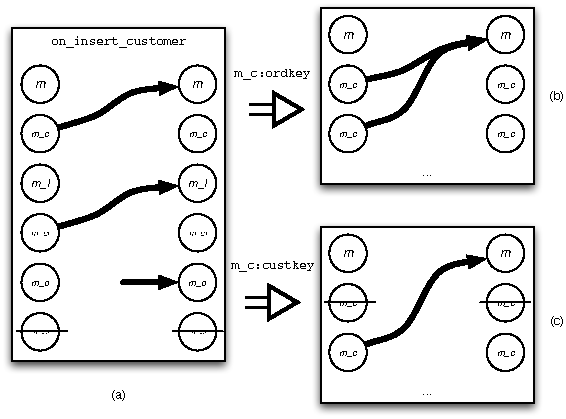
\includegraphics[width=2.5in]{graphics/MessagingGraph}
\end{center}
\caption{An example of a messaging graph based on Section \ref{sec:dbtoaster}'s example query.  (a) The messaging graph for the \texttt{on\_insert\_customer} event.  (b) The effects of splitting view $m_c$ on \texttt{ordkey}.  (c) The effects of splitting $m_c$ on \texttt{custkey}.}
\label{fig:diag:messagingGraph}
\vspace*{-0.2in}
\end{figure}

For example, consider the transition function that results from an update to the
customer table.  One specific subtask of this transition reads $m_c$ and writes
to $m$.  Treating each view as a node, this task has one edge with one read node
and one write node.

DBToaster considers database layout in terms of how it partitions data across a
physical medium (i.e., memory, disk pages, or a cluster).  Viewed through the
messaging graph, a partitioning is an assignment of all nodes in the graph to
one (or more, in the case of replication) partition.  For example, if they were
small enough, $m$ and $m_c$ might be placed on one disk page each.  Thus, the
subtask requires a read on one page, and an update to a second.

Subdivision of individual views is represented in the messaging graph by
splitting of graph nodes.  Of particular interest is how the new nodes interact
with the hyperedge(s) connected to the original node.  As the split occurs, a
node may stay connected to a hyperedge, the hyperedge may likewise be split, or
in some cases, only one node will remain connected (see Figure
\ref{fig:diag:messagingGraph}b,c).  DBToaster can exploit the limited range of
node split/hyperedge interactions to select an effective partitioning scheme.

For example, when partitioning $m_c$, horizontal partitioning on the value of
\texttt{ordkey} increases the number of nodes connected to the
\texttt{on\_insert\_customer} task edge, while using \texttt{custkey} does not
provoke an increase.  If the data represented by these nodes is split across
multiple disks or servers, the computation must still access all of them.  The
roles are reversed for the \texttt{on\_insert\_order} task edge.  Under (the
false) assumption that both insert events occur with identical frequency,
DBToaster can partition on both keys to minimize the number of connected nodes.

Additional knowledge about the dataset enhances the messaging graph produced by
DBToaster.  For instance, the E-R diagram can be integrated into the messaging
graph; the chain of foreign key dependencies in $q$ is strictly hierarchical. 
DBToaster uses this information and creates partitions along a single axis with
a secondary index to bound the number of partitions accessed by each update
subtask, with respect to the total number of partitions generated.  Similarly,
this information is used by DBToaster to select a partitioning scheme that
places nodes typically connected by a subtask into a single partition; this is
analagous to co-clustering in a traditional DBMS.



\section{DBToaster in the Cloud}
\label{sec:distribution}
Scaling up a DDMS requires not only storing progressively more data, but also a
dramatic increase in computing resources.  As alluded to in Section
\ref{sec:storage}, DDMS are amenable to having their data distributed across a
cluster.  We have implemented a cluster-based runtime as part of DBToaster.

\comment{Unlike ad-hoc query systems [MapReduce,HDFS], a distributed DDMS can use advance knowledge of the data usage patterns to better coordinate the distribution of processing with its data placement scheme}

DBToaster considers two general techniques for distributing data and
computation: (1) Compute the data where it will be stored, or (2) Store the data
where it will be used.  The latter approach necessitates potentially extensive
replication of data across the cluster, but enables the use of optimistic
computation techniques that substantially reduce computational latency.

\medspace 

{\bf Creating a total order}\/.
The total ordering of transitions between database steps provides DBToaster with
a clean synchronization abstraction; Each transition is conditioned on the prior
state of the database and potential inter-transition conflicts are known at
compile time.  Unfortunately, imposing such a total ordering in a distributed
setting is not straightforward.  Clients trying to trigger updates in parallel
will easily overwhelm a centralized sorting node, at least at the scales we are
interested in.

Instead, DBToaster imposes a logical total ordering by combining rough clock
synchronization with an arbitrary total ordering over the clients.  The total
ordering ensures that a transition sees only the effects of prior transitions,
though it may not see all of them.  This forces DBToaster to support
out-of-order updates, by optimistically applying the transition and recomputing
those portions later changed by transitions occurring earlier in the logical
ordering.

\medspace

{\bf Hybrid consistency}\/.
DBToaster's out-of-order mechanism implements an eventual consistency model that
may not be sufficient for all data processing tasks.  DBToaster uses a
background task to periodically identify the furthest point in the update stream
that has been fully propagated, and produces a consistent snapshot from the data
at that point.  Interestingly, this background task is already necessary for
garbage collection.  Thus, the same system can simultaneously produce a
low-latency eventually consistent agile view, as well as a periodic consistent
snapshot of the same data, an interface similar to that provided
by~\cite{bayou}.

\medspace

{\bf Availability}\/.
One other interesting point in the distributed design space is that of
availability and recovery.
%Traditional stream processors dwell entirely in-memory for efficiency reasons, and rely on replication-based strategies to provide high availability.  Conversely, t
The large state found in a DDMS necessitates the use of out-of-core storage. 
Instead of over-provisioning replicas and consuming precious network bandwidth
maintaining them, DBToaster can ensure recoverability by maintaining data in a
persistent store.  Tuning the tradeoffs between these various options, however,
remains an open issue.


\section{Discussion and Conclusions}
We have proposed Dynamic Data Management Systems,
arguing for the need for a class of systems optimized
for keeping SQL aggregate views highly available and fresh under
high update rates.
We have sketched some of the main research challenges in
making DDMS a reality, and have outlined key design decisions
and first results and insights that make us confident that
the vision of DDMS can be realized.

We are currently developing a DDMS, DBToaster, in a collaboration
between EPFL and Johns Hopkins, which was started while the
authors worked at Cornell.
%
So far, we have developed an initial version of a
transition compiler which implements the recursive IVM technique
sketched in Section~\ref{sec:compilation}. The feasibility of
keeping views fresh through hundreds of updates per second using
this approach in the context of algorithmic trading
was recently demonstrated using an early DBToaster prototype
\cite{ahmad-vldb:09}. An initial account of the foundations and
theory of recursive IVM was given in \cite{koch-pods:10}.
We are now working on the actual DBToaster DDMS. We follow the
strategy of developing two branches, one a main-memory, moderate
state-size, single-core ultra-high view refresh rate system for
applications such as algorithmic trading and the other
a cloud-based, persistent, eventual-consistency system for
very large scale interactive data analysis. We will
merge these two branches once the individual technical
problems have been solved.


\comment{
Current ongoing research and development directions in
the DBToaster project include: i) leveraging
structural recursion to build a main-memory query processing library based on
functional programming techniques (see Section~\ref{sec:compilation}); ii)
parallelization, deployment and experimentation of a continuous analytics engine
in a cloud environment; iii) analysing the benefits of our execution model in a
batch operating mode on top of map-reduce.
} % 


\scriptsize{
\bibliographystyle{abbrv}
\bibliography{ref}
}



\end{document}
